\documentclass[conference,harvard,brazil,english]{sbatex}
\usepackage[T1]{fontenc}
\usepackage{textcomp}
\usepackage[utf8]{inputenc}
\usepackage{graphicx}
\usepackage{url}
\usepackage{bbding}
\usepackage{fixltx2e}

\graphicspath{{images/}}
	
\begin{document}
	\title{Comparação de algoritmos de detecção de bordas}
	\author{Manoel Vieira Coelho Neto}{vieiranetoc@gmail.com}
	\address{SQS 203 Bloco J\\ Brasília, DF, Brasil}
	
	\twocolumn[{
		\maketitle		
	}]
	\selectlanguage{Brazil}
	\section{Objetivos}
	\par Este relatório tem como objetivo apresentar os resultados para comparação de diferentes algoritmos de detecção de bordas em relação com um um \textit{ground truth} de referência. Assim, aplicamos o método de Solbel, Laplace e Canny para detecção de bordas e comparamos a porcentagem de igualdade entre a saída do algoritmo e o \textit{ground truth}.
	
	\section{Introdução}
		\par Três algoritmos foram usados para detecção de bordas: Sobel, Laplace e Canny.
		\par Para o operador de Sobel, calculamos as derivadas horizontais e verticais dos pixeis da imagem e então tiramos o gradiente G dado por $G = |G\textsubscript{x}|+|G\textsubscript{y}|$ em que:\newline
			\[ G\textsubscript{x} = \left| \begin{array}{ccc}
			\-1 & 0 & +1 \\
			-2 & 0  & +2 \\
			-1 & -0 & +1 \end{array}\right| * I.\]
			
			\[ G\textsubscript{x} = \left| \begin{array}{ccc}
			\-1 & -2 & -1 \\
			0 & 0  & 0 \\
			+1 & +2 & +1 \end{array}\right| * I.\] 
		\par\centerline{Onde I é a imagem a ser operada e } 
		\centerline{$G_x G_y$ são matrizes de convolução}
		\par De fato o operador de Sobel é um operador de diferenciação discreta, simplesmente computa a aproximação do gradiente de uma imagem, combinando borramento gaussiano e diferenciação.
		\par O operador de Laplace se refere à segunda derivada dos pixeis de uma imagem e é um operador de segunda ordem, assim nos pontos de máximos do operador de primeira ordem, a segunda derivada é igual a zero. Então o que deve ocorrer é:\newline
		\centerline{$G' = 0$}
		\par Ou usamos o laplaciano do pixel, dado pela sua derivada em x e y.\newline
		\centerline{$Laplace(f) = \frac{\delta^2f}{\delta x^2} + \frac{\delta^2f}{\delta y^2}$}
		\par Mas ambos os anteriores apesar de fazer um bom trabalho não tem retorno satisfatório em termos de porcentagem de bordas achadas, porque ambos dependem de achar a derivada máxima de um pixel e há um erro associado ao cálculo pois, às vezes acaba-se por achar um máximo local ao invés de um global. Então Canny propôs seu método objetivando três critérios principais:
		\begin{itemize}
			\item Baixa taxa de erro: Boa detecção somente em bordas existentes
			\item Boa localização: a distância entre pixeis de bordas detectados e os reais tem de ser minimizadas.
			\item Resposta Mínima: Somente uma resposta de detector por borda.
		\end{itemize}
		\par O primeiro passo é usar um filtro gaussiano para reduzir o ruído da imagem
		\par Achar o gradiente da imagem, usando um método análogo ao de Sobel, após calcular as matrizes de convolução, após isso, tira-se a magnitude de G, e sua direção $\theta$, onde:
		\centerline{$\theta = arctan(\frac{G_y}{G_x})$}
		\par E a direção é dada em 4 possíveis ângulos: 0°, 45°, 90° ou 135°.
		\par Aplica-se a supressão de não-máximos, removendo todos os pixeis que não são considerados parte de uma borda, assim, somente as linhas finas, que são nesse caso as linhas de interesse - borda - restarão na imagem.
		\par E o passo final é chamado de histerese, onde são aplicados dois \textit{thresholds}, o primeiro verifica se o pixel está acima do valor de \textit{threshold}, se sim, é aceito como uma borda, se não é rejeitado e o segundo verifica se os pixeis que estão entre os dois valores estão conectados a uma borda, se sim são bordas, se não, são rejeitados.
	\section{Metodologia}
		Os algoritmos de Sobel, Operador de Laplace e Canny usados foram os que estão implementados no site de tutoriais do OpenCV e podem ser verificados nas urls abaixo.\newline\newline
		\url{http://docs.opencv.org/doc/tutorials/imgproc/imgtrans/sobel_derivatives/sobel_derivatives.html}\newline
		\url{http://docs.opencv.org/doc/tutorials/imgproc/imgtrans/canny_detector/canny_detector.html}\newline
		\url{http://docs.opencv.org/doc/tutorials/imgproc/imgtrans/laplace_operator/laplace_operator.html}\newline
		
		\par E aplicando-se cada um dos filtros a imagens de exemplo e por fim comparando pixel a pixel a saída com sua \textit{ground truth}, fazemos uma porcentagem de pixeis correspondentes entre as duas, para que se possa analisar qual o melhor método de detecção de bordas.
		
	\section{Resultados}
		Para a imagem de entrada:\newline\newline
		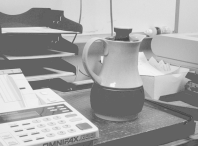
\includegraphics{46.png}\newline\newline\newline
		Temos as seguintes saídas:\newline\newline
		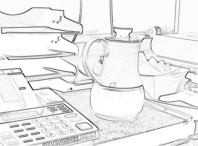
\includegraphics{sob46binarized.png}
		\centerline{Sobel}\newline\newline\newline
		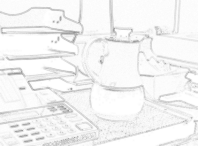
\includegraphics{lapla46binarized.png}
		\centerline{Laplace}\newline\newline\newline
		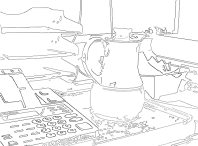
\includegraphics{Canny46binarized.png}
		\centerline{Canny}\newline\newline\newline
		\par Nossa imagem de \textit{ground truth} que nos da as bordas "reais" da imagem é:\newline\newline\newline
		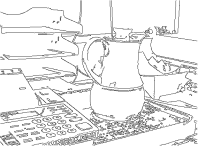
\includegraphics{46gt.png}
		\par Fazendo a comparação 1-1 de cada uma das saídas com o \textit{ground truth} para todas as imagens de exemplo temos a seguinte tabela de porcentagem de correspondência:
		\begin{table}[h]
			\centering
			\caption{Precisão dos algortimos}
			\label{my-label}
			\begin{tabular}{lllllll}
				Precisão & 46 & 140 & 208 & 212 & 217 & 221 \\
				Sobel    & 0.2&0.006& 0.01&0.006& 0.01& 0.10\\
				Laplace  & 0.3& 0.07& 0.05& 0.11& 0.09& 0.20\\
				Canny    & 0.9&0.75 & 0.76& 0.76& 0.72& 0.88
			\end{tabular}
		\end{table}
		\section{Conclusão e Discussões}
			Assim foi constatado a maior precisão do operador de Canny. De fato há mais cuidado sobre os resultados do gradiente e a suavização de ruídos que possam atrapalhar. Para imagens com uma variação muito alta de cor entre duas regiões é possível perceber que até mesmo Canny tem um certo nível de falha, uma vez que todos os operadores aplicados no presente processo dependem do gradiente, que nada mais é que a derivada do pixel em x e y. Então, caso haja uma variação brusca, o filtro tende a ser impreciso naquela região de variação.
		\bibliography{exemplo}
		\cite{docsocv}\newline
		\url{http://docs.opencv.org/doc/tutorials/imgproc/imgtrans/sobel_derivatives/sobel_derivatives.html}\newline
		\url{http://docs.opencv.org/doc/tutorials/imgproc/imgtrans/canny_detector/canny_detector.html}\newline
		\url{http://docs.opencv.org/doc/tutorials/imgproc/imgtrans/laplace_operator/laplace_operator.html}\newline
	
\end{document}
